\documentclass[11pt]{article}
\usepackage[margin=0.8in]{geometry}
\usepackage{booktabs}
\usepackage{graphicx}
\usepackage{hyperref}
\usepackage{xurl}
\usepackage{microtype}
\usepackage{float}
\hypersetup{colorlinks=true,urlcolor=blue,citecolor=blue,linkcolor=blue}
\title{What a Popular PCOS Dataset Misses in the PMOS Era}
\author{PMOS Research Team}
\date{\today}
\begin{document}
\maketitle

\section*{Plain-English Summary}
PCOS has been renamed polyendocrine metabolic ovarian syndrome (PMOS). The new name matters because it points away from a narrow ovarian-cyst framing and toward a lifelong endocrine and metabolic condition. The Kaggle dataset is useful for classroom statistics and exploratory modeling, but it was built around the older PCOS measurement frame.

\section*{What the Dataset Covers}
\begin{table}[H]
\caption{PMOS domain coverage in the Kaggle dataset.}
\label{tab:public-coverage}
\small\resizebox{\columnwidth}{!}{\begin{tabular}{lll}
\toprule
PMOS domain & Coverage & Major gaps \\
\midrule
Reproductive / ovarian & Strong & diagnostic visit notes and formal phenotype labels \\
Endocrine & Partial & testosterone, SHBG, DHEAS, free androgen index \\
Metabolic / cardiovascular & Weak proxy & fasting insulin, fasting glucose, HOMA-IR, OGTT, lipids \\
Dermatological / symptoms & Partial & standardized hirsutism/acne scales \\
Psychological / quality of life & Absent & depression, anxiety, sleep, stigma, quality-of-life scales \\
\bottomrule
\end{tabular}}
\end{table}


\begin{figure}[H]
\centering
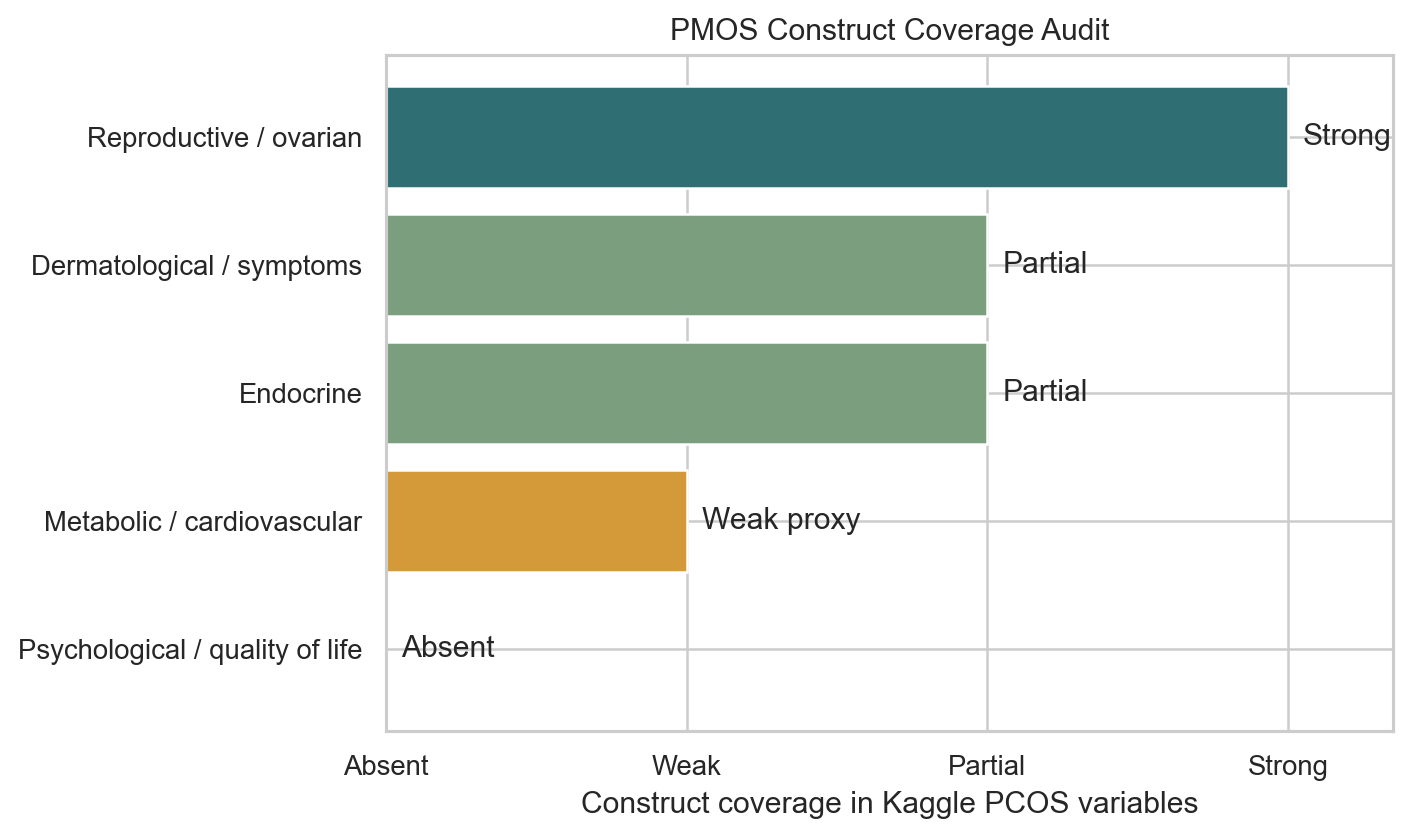
\includegraphics[width=0.86\linewidth]{../figures/pmos_construct_coverage.png}
\caption{The dataset is strongest on reproductive/ovarian variables and weakest on metabolic and psychological PMOS domains.}
\end{figure}

\section*{What the BMI Analysis Adds}
In the PCOS-positive subset, mean BMI was 25.47. The clinical-only BMI model had adjusted $R^2=0.257$, while the laboratory-only model had adjusted $R^2=-0.008$. The clearest predictor was self-reported weight gain.

This is not evidence that hormones or metabolism are unimportant. It is evidence that this public dataset is missing direct metabolic biosignals such as fasting insulin, fasting glucose, HOMA-IR, OGTT, lipids, and testosterone.

\section*{Classification Context}
We also ran two simple logistic classifiers for PCOS/PMOS status. These are not diagnostic tools; they show what kind of signal the dataset contains.

\begin{table}[H]
\caption{Classifier context results.}
\label{tab:public-classifiers}
\small\resizebox{\columnwidth}{!}{\begin{tabular}{lrrrrr}
\toprule
Model & Test n & AUC & Brier score & Sensitivity & Specificity \\
\midrule
Ovary-centric & 162 & 0.919 & 0.106 & 0.792 & 0.899 \\
Metabolic + symptom & 162 & 0.860 & 0.135 & 0.736 & 0.881 \\
\bottomrule
\end{tabular}}
\end{table}


\begin{figure}[H]
\centering
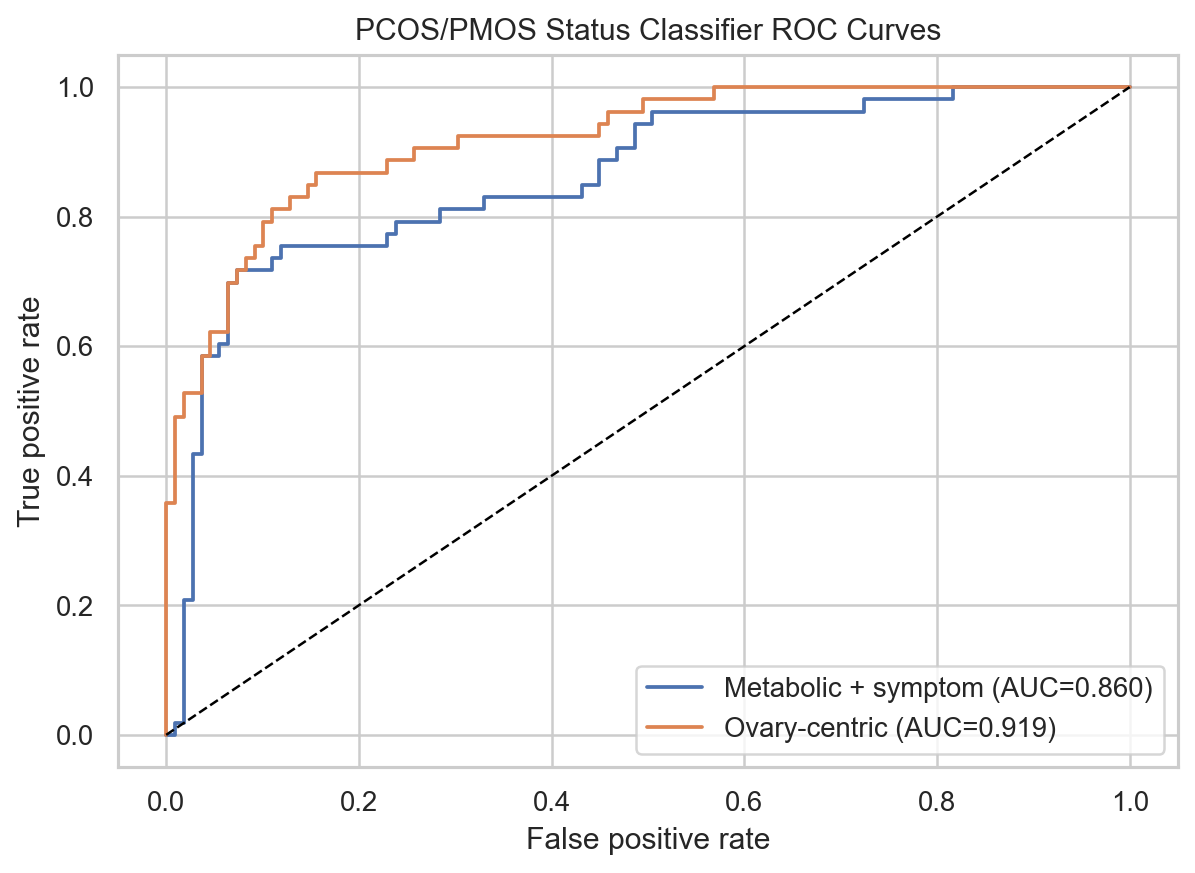
\includegraphics[width=0.72\linewidth]{../figures/classifier_roc_curves.png}
\caption{ROC curves for two PCOS/PMOS-status classifiers.}
\end{figure}

\begin{figure}[H]
\centering
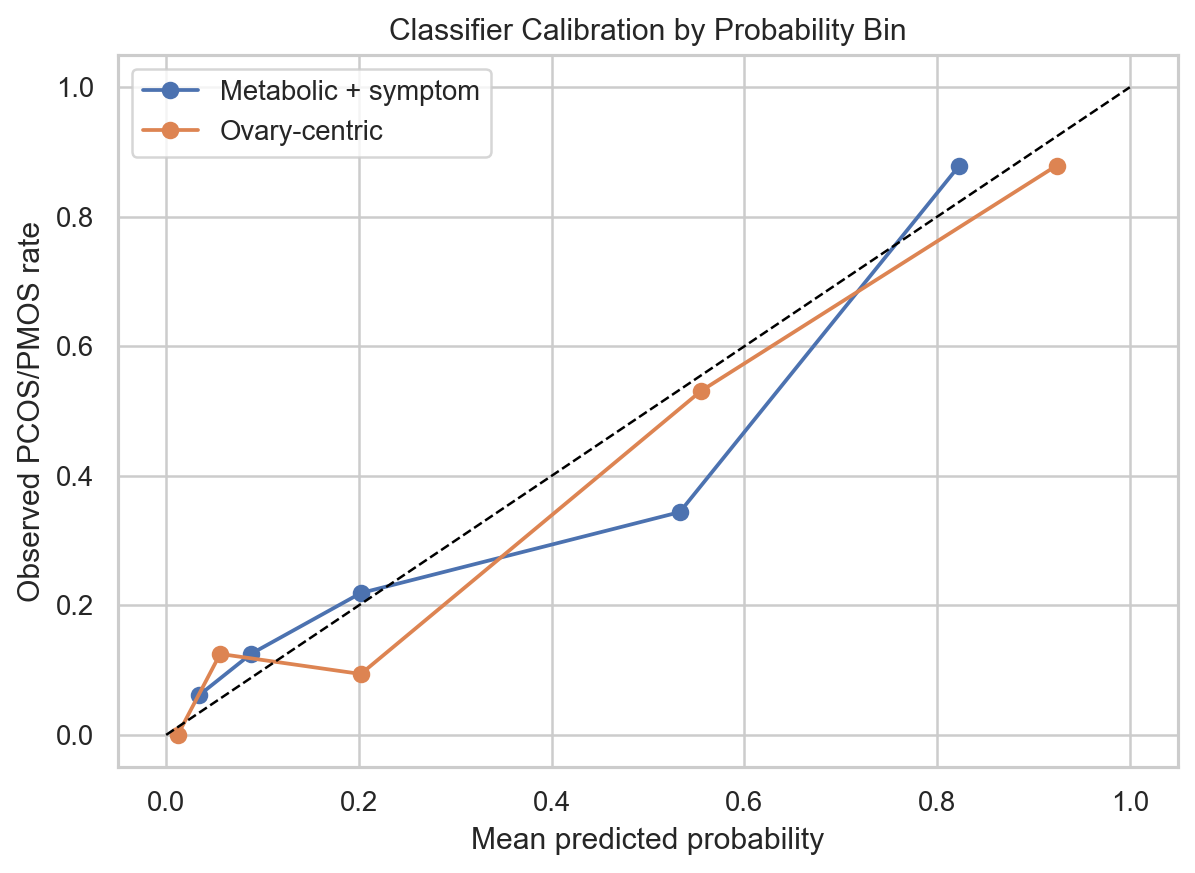
\includegraphics[width=0.72\linewidth]{../figures/classifier_calibration.png}
\caption{Calibration curves by predicted-probability bin.}
\end{figure}

\section*{Public Takeaway}
A dataset can only teach what it measures. This Kaggle dataset can support exploratory PCOS-status modeling, but it cannot fully represent PMOS as a polyendocrine metabolic condition. Future PMOS datasets should include fasting insulin, fasting glucose, HOMA-IR, lipids, blood pressure, androgen assays, mental-health scales, and longitudinal follow-up.

\section*{Source Links}
\begin{itemize}
\item Endocrine Society PMOS release: \url{https://www.endocrine.org/news-and-advocacy/news-room/2026/pcos-name-change}
\item Monash PMOS release: \url{https://www.monash.edu/medicine/news/latest/2026-articles/polyendocrine-metabolic-ovarian-syndrome-new-name-to-improve-diagnosis-and-care-of-condition-affecting-170-million-women-worldwide}
\item Kaggle dataset: \url{https://www.kaggle.com/datasets/prasoonkottarathil/polycystic-ovary-syndrome-pcos}
\end{itemize}
\end{document}
